\documentclass[11pt, a4paper]{article}

% ── Packages ──────────────────────────────────────────────────────────────
\usepackage[utf8]{inputenc}
\usepackage[T1]{fontenc}
\usepackage{amsmath, amssymb}
\usepackage{physics}
\usepackage{graphicx}
\usepackage{hyperref}
\usepackage{booktabs}
\usepackage{xcolor}
\usepackage{tcolorbox}
\usepackage{listings}
\usepackage{geometry}
\usepackage{caption}
\usepackage{tikz}
\usepackage{soul}            % for \hl highlighting
\usepackage{marginnote}
\usepackage{mdframed}
\usetikzlibrary{positioning, arrows.meta, calc}

\geometry{margin=1in, marginparwidth=0.8in}
\hypersetup{colorlinks=true, linkcolor=blue!70!black, urlcolor=blue!60!black}

\tcbset{
  nb/.style={colback=yellow!8!white, colframe=orange!60!black,
             boxrule=0.4pt, left=4pt, right=4pt, top=2pt, bottom=2pt},
  imp/.style={colback=red!5!white, colframe=red!50!black,
              boxrule=0.4pt, left=4pt, right=4pt, top=2pt, bottom=2pt},
  code/.style={colback=gray!5!white, colframe=gray!40!black,
               boxrule=0.4pt, left=4pt, right=4pt, top=2pt, bottom=2pt}
}

\lstset{
    language=Python,
    basicstyle=\ttfamily\small,
    keywordstyle=\color{blue!70!black}\bfseries,
    commentstyle=\color{green!50!black}\itshape,
    stringstyle=\color{red!60!black},
    numbers=left, numberstyle=\tiny\color{gray},
    breaklines=true, frame=single,
    backgroundcolor=\color{gray!5},
    showstringspaces=false
}

% quick command for margin scribbles
\newcommand{\sidenote}[1]{\marginnote{\scriptsize\textit{#1}}}

% ══════════════════════════════════════════════════════════════════════════
\title{Notes on TrackHHL / 1-Bit Quantum Filter\\[4pt]
       \large Chiotopoulos et al.\ --- arXiv:2511.11458}
\author{my notes}
\date{}

\begin{document}
\maketitle

\noindent\textit{These are my notes from reading the TrackHHL paper and
running the example notebook. Trying to break everything down so I actually
understand what's going on.}

\bigskip
\hrule
\tableofcontents
\hrule
\newpage

% ══════════════════════════════════════════════════════════════════════════
\section{Ok so what is this actually about}

The short version: at the LHC (the big particle collider at CERN), protons
get smashed together and a ton of new particles fly out. These particles pass
through layers of silicon detectors and leave little signals called
\textbf{hits}. The problem is figuring out which hits came from the same
particle --- i.e.\ connecting the dots into \textbf{tracks}.

\begin{center}
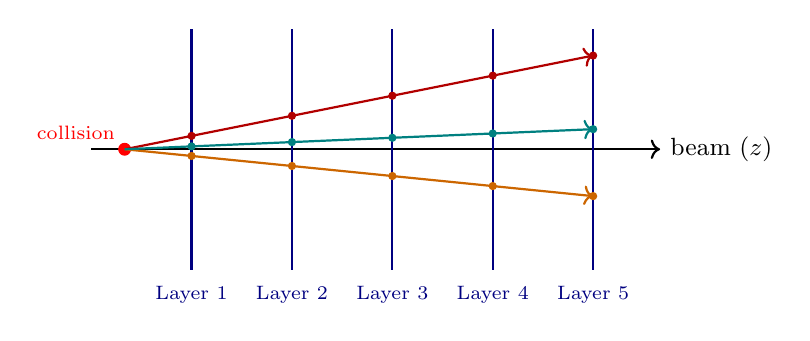
\begin{tikzpicture}[scale=0.85]
  \draw[thick, ->] (-0.5,0) -- (8,0) node[right]{\small beam ($z$)};
  \foreach \x/\lbl in {1/1, 2.5/2, 4/3, 5.5/4, 7/5} {
    \draw[thick, blue!50!black] (\x,-1.8) -- (\x,1.8);
    \node[below, blue!50!black, font=\scriptsize] at (\x,-1.9) {Layer \lbl};
  }
  \filldraw[red] (0,0) circle (2.5pt) node[above left, font=\scriptsize]{collision};
  \draw[thick, red!70!black, ->] (0,0) -- (7, 1.4);
  \draw[thick, orange!80!black, ->] (0,0) -- (7, -0.7);
  \draw[thick, teal, ->] (0,0) -- (7, 0.3);
  \foreach \x in {1, 2.5, 4, 5.5, 7} {
    \filldraw[red!70!black] (\x,{1.4*\x/7}) circle (1.5pt);
    \filldraw[orange!80!black] (\x,{-0.7*\x/7}) circle (1.5pt);
    \filldraw[teal] (\x,{0.3*\x/7}) circle (1.5pt);
  }
\end{tikzpicture}
\end{center}

This is the LHCb \textbf{VELO} detector --- it's the one closest to the
collision point (like 5mm away). It has silicon pixel layers, and since
there's basically no magnetic field there, the tracks are just straight
lines. That makes it a nice test case.

\medskip
The problem is that at the future HL-LHC there'll be $\sim$1500 particles
per event, each leaving $\sim$5 hits. You have to check every possible pair
of hits in neighboring layers, so the number of candidate line segments goes
like $N_{\text{particles}}^2 \times N_{\text{layers}}$. That's millions of
candidates, and it grows \emph{quadratically} with the number of particles.
Current computers are going to struggle.

\medskip
\textbf{The idea in this paper:} turn the tracking problem into solving a
linear system $A\vec{S} = \vec{b}$, then use a quantum algorithm (HHL) to
solve it exponentially faster. But vanilla HHL has way too deep circuits, so
they came up with a simplified ``1-Bit'' version that cuts the circuit size
by a factor of $\sim$1000.

% ══════════════════════════════════════════════════════════════════════════
\newpage
\section{The math --- how tracking becomes a linear system}

\subsection{Segments (doublets)}

A \textbf{segment} (or ``doublet'') = a straight line connecting a hit in
layer $\ell$ to a hit in layer $\ell+1$. We give each one a label $S_i$
where:
\[
  S_i = \begin{cases} 1 & \text{segment is part of a real track} \\
                       0 & \text{it's fake / noise} \end{cases}
\]

Quick example: 2 particles, 3 layers. Each layer has 2 hits. Between
layers 1--2 there are $2 \times 2 = 4$ possible segments, same for layers
2--3, so 8 total. Only 4 are real (2 per particle $\times$ 2 gaps).

In the notebook they use 64 particles and 5 layers, which gives
$64^2 \times 4 = 16{,}384$ segments. Yeah.

\subsection{The Hamiltonian}

We want an energy function that's lowest when the right segments are ``on.''
It has three pieces:

\begin{equation}
  \boxed{H(\vec{S}) = H_{\text{ang}}(\vec{S}, \epsilon) +
  \alpha\, H_{\text{spec}}(\vec{S}) + \beta\, H_{\text{gap}}(\vec{S})}
\end{equation}

Let me go through each one.

\subsubsection{Angular term --- the important one}

\begin{equation}
  H_{\text{ang}} = -\frac{1}{2}\sum_{a,b,c}
  f(\theta_{abc},\epsilon)\, S_{ab}\, S_{bc}
\end{equation}

where $\theta_{abc}$ is the angle between segment $S_{ab}$ and $S_{bc}$
(they share the middle hit $b$), and

\[
  f(\theta_{abc}, \epsilon) = \begin{cases}
    1 & \text{if } \cos\theta_{abc} \geq 1 - \epsilon \\
    0 & \text{otherwise} \end{cases}
\]

\begin{tcolorbox}[nb]
\textbf{What this does:} if two consecutive segments are nearly
collinear (angle $\approx 0^\circ$), their product $S_{ab}S_{bc}$ gets a
$-1/2$ contribution. Negative = \emph{lowers} the energy. So the system
\emph{wants} to turn on segments that form straight lines.

The $\epsilon$ parameter controls how strict the alignment has to be. In
the notebook $\epsilon = 10^{-7}$ which is insanely strict --- only
perfectly straight lines pass.
\end{tcolorbox}

\subsubsection{Spectral term --- penalty for being on}

\begin{equation}
  H_{\text{spec}} = \alpha \sum_{ab} S_{ab}^2
\end{equation}

This makes it cost energy to turn a segment on. Without the angular reward,
everything would prefer to be off. In the notebook $\alpha = 2.0$.

\subsubsection{Gap term --- penalty for being off}

\begin{equation}
  H_{\text{gap}} = \beta \sum_{ab}(1 - S_{ab})^2
  = \beta \sum_{ab}(1 - 2S_{ab} + S_{ab}^2)
\end{equation}

This makes it cost energy to be off. So you have two competing penalties ---
$H_{\text{spec}}$ says ``don't be on'' and $H_{\text{gap}}$ says ``don't be
off.'' The angular term breaks the tie: if you're part of a straight line,
the reward from $H_{\text{ang}}$ justifies turning on. In the notebook
$\beta = 1.0$.

\subsection{Getting to $A\vec{S} = \vec{b}$}
\label{sec:linearsys}

$H$ is quadratic in $\vec{S}$. To minimize it, relax $S_i$ from binary
$\{0,1\}$ to continuous reals and set the gradient to zero:

\begin{equation}
  \nabla H = 0 \quad\Longrightarrow\quad A\,\vec{S} = \vec{b}
\end{equation}

where $A = A_{\text{ang}} + A_{\text{spec}} + A_{\text{gap}}$ (from the
quadratic parts) and $\vec{b} = \beta(1,1,\ldots,1)^T$ (from the linear
part of $H_{\text{gap}}$).

\begin{tcolorbox}[nb]
\textbf{Then you threshold.} The solution $\vec{S}$ has real-valued entries.
Apply a cutoff $T = 0.45$: if $S_i > T$ it's a real segment, otherwise
it's noise. Done.
\end{tcolorbox}

\subsection{Properties of $A$ (why HHL works here)}

\begin{itemize}
  \item \textbf{Hermitian} --- it's real symmetric, $A = A^T$
  \item \textbf{Sparse} --- most entries are zero (only connected segments
        interact). For 16,384 segments there are only 16,768 nonzero entries
  \item \textbf{Condition number $\kappa \leq 5$} --- the eigenvalues don't
        spread out much, thanks to the step function in $H_{\text{ang}}$
  \item \textbf{Constant diagonal} --- every diagonal entry $= \alpha +
        \beta = 3.0$. This gets exploited a lot in the circuit
\end{itemize}

These properties are actually really nice for HHL. Sparsity makes the
Hamiltonian simulation efficient, and low $\kappa$ means the algorithm
converges fast.

% ══════════════════════════════════════════════════════════════════════════
\newpage
\section{The quantum algorithm}

\subsection{Quantum refresher (the bare minimum)}

\begin{itemize}
  \item A \textbf{qubit} can be $\ket{0}$, $\ket{1}$, or a superposition:
        $\ket{\psi} = \alpha\ket{0} + \beta\ket{1}$ with
        $|\alpha|^2 + |\beta|^2 = 1$
  \item \textbf{Measurement} collapses it: get $\ket{0}$ with prob
        $|\alpha|^2$, $\ket{1}$ with prob $|\beta|^2$
  \item \textbf{Gates} = unitary matrices on qubits. Important ones:
        Hadamard ($H$), CNOT, $R_x(\theta)$
  \item $n$ qubits $\Rightarrow$ state lives in $2^n$-dimensional space.
        That exponential scaling is the whole point
\end{itemize}

\subsection{Standard HHL --- the 5 steps}

HHL solves $A\vec{x} = \vec{b}$ quantumly. Here's how:

\medskip
\textbf{1) State prep.} Encode $\vec{b}$ as $\ket{b}$. For us $\vec{b} =
(1,1,\ldots,1)^T$ so it's just Hadamard gates on all qubits:
$H^{\otimes n}\ket{0\cdots0} = \frac{1}{\sqrt{2^n}}\sum_i \ket{i}$

\medskip
\textbf{2) Quantum Phase Estimation (QPE).} Decompose $\ket{b}$ in the
eigenbasis of $A$: $\ket{b} = \sum_i c_i \ket{u_i}$ where
$A\ket{u_i} = \lambda_i\ket{u_i}$. QPE writes the eigenvalue into an
ancilla register:
\[
  \sum_i c_i \ket{\tilde\lambda_i}\ket{u_i}
\]

\medskip
\textbf{3) Eigenvalue inversion.} Do a controlled rotation on a fresh
ancilla qubit to encode $1/\lambda_i$ in the amplitude:
\[
  \sum_i c_i \ket{\tilde\lambda_i}\ket{u_i}\left(
  \frac{C}{\lambda_i}\ket{1} + \cdots\ket{0}\right)
\]

\medskip
\textbf{4) Uncompute QPE.} Run QPE backwards to clean up the eigenvalue
register.

\medskip
\textbf{5) Measure.} Post-select on ancilla $= \ket{1}$. What's left is:
$\ket{x} \propto \sum_i \frac{c_i}{\lambda_i}\ket{u_i} = A^{-1}\ket{b}$

\begin{tcolorbox}[imp]
\textbf{Problem 1:} QPE makes the circuit insanely deep. For 5 particles
and 3 layers the naive HHL circuit has \textbf{14.5 million gates}. Not
happening on any real hardware.

\textbf{Problem 2:} The answer is encoded in amplitudes. To read out the
full vector $\vec{S}$ you need $\sim O(N^2)$ measurements, which basically
kills the quantum speedup.
\end{tcolorbox}

\subsection{The 1-Bit Quantum Filter (the actual contribution)}

The paper's fix has two key ideas:

\subsubsection{Idea 1: Coarse Suzuki-Trotter}

QPE needs $e^{iAt}$ which is expensive. The Suzuki-Trotter decomposition
approximates:
\[
  e^{t(A_1+A_2)} \approx \left(e^{tA_1/n}\, e^{tA_2/n}\right)^n
\]

They use $n=1$, $t=1$ --- the crudest possible approximation. Normally this
would be terrible, but here it actually helps:

\begin{tcolorbox}[nb]
With $n=1, t=1$ the Trotter approximation \textbf{suppresses all inactive
segments to zero amplitude}. The output becomes effectively binary ---
exactly what we need. The ``error'' from the coarse approximation is
actually a feature.
\end{tcolorbox}

Since $A$ has a constant diagonal $c = \alpha + \beta$, we can write
$A = cI - B$ and then:
\[
  e^{iAt} \approx e^{ict} \cdot e^{-iBt}
\]
$e^{ict}$ is just a global phase (doesn't affect measurement). $e^{-iBt}$
is implemented as a product of two-qubit Givens rotations, one for each
interacting pair of segments.

\subsubsection{Idea 2: Only 1 bit of phase precision}

Since we just need to know ``active or not'' (binary), we only need to tell
apart ``eigenvalue $\approx 0$'' from ``eigenvalue $\neq 0$.'' One bit of
QPE is enough for that.

This changes the qubit scaling:
\[
  \underbrace{O(2\log_2 N + 2)}_{\text{standard HHL}}
  \quad\longrightarrow\quad
  \underbrace{O(\log_2 N + 3)}_{\text{1-Bit HHL}}
\]

For HL-LHC scale: $\sim$47 qubits $\to$ $\sim$26 qubits.

\subsection{How the circuit actually works}

Three registers:

\begin{center}
\begin{tabular}{lll}
\toprule
Register & Qubits & What it does \\
\midrule
Time    & 1             & the single QPE phase qubit \\
System  & $\log_2 N$    & holds $\ket{b}$ / the solution \\
Ancilla & 1             & post-selection flag \\
\bottomrule
\end{tabular}
\end{center}

\medskip
The circuit goes:

\begin{enumerate}
  \item $H$ on all system qubits $\to$ prepare $\ket{b} \propto
        (1,1,\ldots)^T$
  \item $H$ on time qubit, then controlled-$e^{iAt}$ (Trotter), then
        inverse QFT on time qubit (for 1 qubit, IQFT is just $H$ again)
        --- this is the 1-bit QPE
  \item $X$--CNOT--$X$ gadget: flips the ancilla when time qubit $=
        \ket{0}$
  \item Uncompute QPE (run step 2 backwards)
  \item Measure everything
\end{enumerate}

\begin{tcolorbox}[nb]
\textbf{Why does the ancilla trick work?}

After Trotter QPE:
\begin{itemize}
  \item Active segments $\to$ eigenvalue near the big eigenvalue $\to$
        phase $\approx 0$ $\to$ time qubit $= \ket{0}$
  \item Inactive segments $\to$ eigenvalue $\approx 0$ $\to$ phase
        $\approx 1$ $\to$ time qubit $= \ket{1}$
\end{itemize}
The $X$-CNOT-$X$ flips ancilla only when time $= \ket{0}$, so
post-selecting on ancilla $= \ket{1}$ keeps only the active segments.
Pretty clever.
\end{tcolorbox}

\subsection{How much better is this?}

For 5 particles, 3 layers (14 qubits), transpiled for IBM hardware:

\begin{center}
\begin{tabular}{lrrr}
\toprule
Method & Total Gates & 2-Qubit Gates & Reduction \\
\midrule
Naive HHL           & 14,515,229 & 7,107,317 & $1\times$ \\
Qiskit O3           & 1,089,295  & 501,066   & $13\times$ \\
+ Trotter           & 257,367    & 120,171   & $56\times$ \\
\textbf{+ 1-Bit PE} & \textbf{11,547} & \textbf{8,780} &
  $\mathbf{\sim 1{,}000\times}$ \\
\bottomrule
\end{tabular}
\end{center}

\sidenote{$10^3$--$10^4$ reduction depending on event size}

That's \emph{three orders of magnitude} fewer gates. Also reduces the
number of samples needed from $\sim$10 million to $\sim$10 thousand (for
HL-LHC conditions) because the suppressed inactive segments don't need to
be measured.

% ══════════════════════════════════════════════════════════════════════════
\newpage
\section{Walking through the notebook}

Ok now let me go through what the code actually does cell by cell.

\subsection{Imports}

\begin{lstlisting}
from toy_model import state_event_model
from toy_model.state_event_generator import *
from toy_model.simple_hamiltonian import SimpleHamiltonian
from toy_model.utils import plot_solution_comparison, plot_event_2d
from quantum_algorithms.OneBQF import OneBQF as onebqf
import numpy as np
\end{lstlisting}

Three modules: the toy detector/event simulator, the Hamiltonian builder,
and the quantum solver.

\subsection{Setting up the detector and events}

\begin{lstlisting}
dz = 20                 # 20mm between layers
n_particles = [64]      # 64 particles
layers = 5              # 5 detector layers

# each layer is 33x33mm
lx = [33 for x in range(1, layers+1)]
ly = [33 for x in range(1, layers+1)]
zs = [dz*l for l in range(1, layers+1)]  # z = 20,40,60,80,100
\end{lstlisting}

Then it generates 64 particles from a single collision point, propagates
them through 5 layers (giving 320 hits total), and builds all possible
segments between adjacent layers.

\begin{tcolorbox}[nb]
Between each pair of layers: $64 \times 64 = 4{,}096$ candidate segments.
$\times\, 4$ gaps $= 16{,}384$ total segments. So the Hamiltonian matrix
$A$ is $16{,}384 \times 16{,}384$. But it's super sparse --- only 16,768
nonzero entries out of $\sim$268 million.
\end{tcolorbox}

\subsection{Building and running the quantum circuit}

\begin{lstlisting}
A = ham.A.todense()
vector_b = np.ones(len(A))

hhl_solver = onebqf(matrix_A, vector_b,
    num_time_qubits=1,   # <-- THE 1 BIT
    shots=10000,
    debug=False)

circuit = hhl_solver.build_circuit()
counts = hhl_solver.run(use_noise_model=False)
quantum_solution, total_success = hhl_solver.get_solution()
\end{lstlisting}

\texttt{num\_time\_qubits=1} is the whole point --- one qubit for phase
estimation instead of many. \texttt{shots=10000} means run the circuit
10,000 times. \texttt{use\_noise\_model=False} means perfect simulation
(no hardware noise).

\medskip
Under the hood, \texttt{get\_solution()} does:
\begin{enumerate}
  \item Filter for measurements where ancilla $= \ket{1}$ (post-selection)
  \item Count occurrences of each system state $\to$ probabilities $p_i$
  \item Take $\sqrt{p_i}$ to get amplitudes (measurement gives
        $|\text{amplitude}|^2$)
  \item Normalize
\end{enumerate}

\subsection{Checking the answer}

\begin{lstlisting}
classical_solution = ham.solve_classicaly()  # conjugate gradient
T = .45
discretized = (classical_solution > T).astype(int)

set1 = set(np.nonzero(discretized)[0])
set2 = set(np.nonzero(quantum_solution)[0])
print("Solutions match", set1 - set2)
\end{lstlisting}

Output: \texttt{Solutions match set()}

\begin{tcolorbox}[nb]
Empty set = every segment the classical solver said was active, the
quantum solver also said was active. \textbf{Perfect match.}
\end{tcolorbox}

\subsection{Circuit stats}

After decomposing the circuit all the way down to basic gates:

\begin{verbatim}
Circuit Depth: 507
Circuit Statistics: {'u': 365, 'cx': 321, 'u3': 144, 'measure': 6}
\end{verbatim}

So depth 507 (longest sequential chain), 321 CNOT gates (the expensive
two-qubit ones), and 509 single-qubit rotations. For a 16,384-dimensional
linear system, that's absurdly shallow. Only needs 7 qubits total
(1 time + 5 system + 1 ancilla).

\subsection{TKET optimization}

They also ran the circuit through TKET (Quantinuum's compiler) which
does peephole optimization --- combining/canceling adjacent gates:

\begin{verbatim}
Gates: Counter({OpType.CX: 321, OpType.TK1: 310, OpType.Measure: 6})
Depth: 439
\end{verbatim}

Depth goes from 507 $\to$ 439 (about 13\% reduction). CX count stays at
321 --- it was already close to optimal.

% ══════════════════════════════════════════════════════════════════════════
\newpage
\section{Results summary}

\subsection{It works}

For 64 particles / 5 layers / 16,384 segments, the 1-Bit Quantum Filter
finds the exact same active segments as the classical solver. Zero
mismatches. The quantum solution perfectly reconstructs all particle tracks.

\subsection{Circuit is actually feasible}

\begin{center}
\begin{tabular}{lcc}
\toprule
& Standard HHL & 1-Bit HHL \\
\midrule
Qubit scaling & $O(2\log_2 N + 2)$ & $O(\log_2 N + 3)$ \\
HL-LHC qubits & $\sim$47 & $\sim$26 \\
Gate reduction & $1\times$ & $\sim 10^3\times$ \\
\bottomrule
\end{tabular}
\end{center}

\subsection{Fewer measurements needed}

Because inactive segments are suppressed, sampling requirements drop:
\[
  \underbrace{O(N_p^2 \cdot N_h \cdot \log(N_p^2 \cdot N_h))}_{\text{standard HHL}}
  \quad\to\quad
  \underbrace{O(N_p \cdot N_h \cdot \log(N_p \cdot N_h))}_{\text{1-Bit HHL}}
\]

For 1500 particles: $\sim$10 million $\to$ $\sim$10 thousand queries. And
the paper shows you can reconstruct Primary Vertices with only $\sim$40\%
of the segments, reducing this even further.

% ══════════════════════════════════════════════════════════════════════════
\section{Caveats / things to keep in mind}

\begin{itemize}
  \item Everything here ran on a \textbf{noiseless simulator}. Real quantum
        hardware has gate errors, decoherence, crosstalk, etc. The paper
        does test IBM noise models (Torino, Marrakesh, Pittsburgh, Fez) and
        Quantinuum emulators separately

  \item The toy model is idealized --- 100\% detector efficiency, perfectly
        straight tracks, no scattering. Real detectors are messier

  \item Even with suppression, reading out the full track solution still
        requires a lot of measurements. The paper's workaround: reconstruct
        just the Primary Vertices instead, which needs way fewer samples

  \item 26 qubits is more realistic than 47 but the circuit depth for 1500
        particles is still a challenge. They mention Quantum Singular Value
        Transform as something to explore next
\end{itemize}

% ══════════════════════════════════════════════════════════════════════════
\section{Main takeaways}

\begin{enumerate}
  \item Track reconstruction $\to$ minimize a Hamiltonian $\to$ solve a
        linear system $A\vec{S} = \vec{b}$

  \item HHL quantum algorithm solves linear systems with exponential
        speedup in theory, but the circuits are way too deep in practice

  \item The \textbf{1-Bit Quantum Filter} fixes this by:
  \begin{itemize}
    \item Using a coarse Suzuki-Trotter that happens to suppress noise
          segments
    \item Only needing 1 bit of phase estimation since the problem is
          binary
    \item Result: $\sim$1000$\times$ fewer gates, half the qubits, way
          fewer measurements
  \end{itemize}

  \item The notebook shows the full pipeline working: simulate
        $\to$ build Hamiltonian $\to$ quantum solve $\to$ exact match with
        classical answer

  \item Not ready for real hardware at LHC scale yet, but it's a solid
        proof of concept
\end{enumerate}

% ══════════════════════════════════════════════════════════════════════════
\newpage
\section*{Glossary}

\begin{tabular}{ll}
\toprule
Term & What it means \\
\midrule
LHC & Large Hadron Collider (the big ring at CERN) \\
HL-LHC & High-Luminosity LHC (future upgrade, way more collisions) \\
LHCb & one of the 4 main LHC experiments \\
VELO & Vertex Locator (sub-detector closest to collision) \\
PV & Primary Vertex (the collision point) \\
Hit & signal from a particle crossing a detector layer \\
Segment/Doublet & line between two hits in adjacent layers \\
HHL & Harrow-Hassidim-Lloyd (quantum linear systems algorithm) \\
QPE & Quantum Phase Estimation \\
QFT & Quantum Fourier Transform \\
CX/CNOT & Controlled-NOT gate (2-qubit gate) \\
Ancilla & auxiliary qubit used for post-selection \\
$\kappa$ & condition number $= \lambda_{\max}/\lambda_{\min}$ \\
TKET & Quantinuum's quantum circuit compiler \\
\bottomrule
\end{tabular}

\bigskip
\noindent\textbf{References:}
\begin{itemize}
  \item Paper: \url{https://arxiv.org/abs/2511.11458}
  \item Code: \url{https://github.com/Xenofon-Chiotopoulos/OneBQF}
  \item Previous work (Nicotra et al.): JINST \textbf{18}, P11028 (2023)
  \item HHL original: Harrow, Hassidim, Lloyd --- PRL \textbf{103}, 150502
        (2009)
\end{itemize}

\end{document}
